\documentclass[aps,pre,reprint,twocolumn,nofootinbib,superscriptaddress]{revtex4-2}

\usepackage{amsmath,amssymb,amsthm}
\usepackage{graphicx}
\usepackage{bm}
\usepackage{xurl}
\usepackage{xcolor}
\usepackage{hyperref}

\hypersetup{
    pdfauthor={Taishi Namba},
    pdftitle={Is the resolution gap of the arrow of time uniform?},
    pdfkeywords={coarse-graining, arrow of time, resolution gap, Fisher information, uncertainty principle, Gaussian smoothing, Hamiltonian dynamics},
    hidelinks
}

\newtheorem{theorem}{Theorem}
\newtheorem{proposition}[theorem]{Proposition}
\newtheorem{lemma}[theorem]{Lemma}
\newtheorem{corollary}[theorem]{Corollary}
\newtheorem{observation}{Numerical result}
\newtheorem{conjecture}{Conjecture}
\theoremstyle{remark}
\newtheorem*{remark}{Remark}

\newcommand{\E}{\mathbb{E}}
\newcommand{\Var}{\operatorname{Var}}
\newcommand{\Cov}{\operatorname{Cov}}
\newcommand{\xb}{\bar{x}_w}
% Draft marker for items still to be filled in. Remove before release.
\newcommand{\pending}[1]{{\color{red}\textbf{[#1]}}}

\begin{document}

\title{Is the resolution gap of the arrow of time uniform?}

\author{Taishi Namba}
\email{neginyan@gmail.com}
\affiliation{Independent Researcher, Atsugi, Kanagawa, Japan}

\date{\today}

\begin{abstract}
An observer who sees a Hamiltonian ensemble through a Gaussian window of width $\sigma$ finds that the coarse-grained entropy grows only if the window widens faster than a critical rate $R$ of the state. For Gaussian states $R$ stays below the largest strain rate $\kappa$ of the flow by a margin proportional to $\sigma$, the resolution gap. We ask whether every state has a gap of order $\sigma$, at the unstable top of the pendulum ($\kappa = 1$). Numerically, it does not. Ripple strips, states that carry a fine ripple along the unstable direction, reach $(\kappa - R)/\sigma = 1/(2k_0)$ as $\sigma \to 0$ for every ripple wavenumber $k_0$ (in units of $1/\sigma$), so that the smallest gap at a given $\sigma$ tends to zero; between $\sigma = 10^{-24}$ and $10^{-96}$ it follows $1.02/\sqrt{\ln(1/\sigma) - 23.4}$, and every value is confirmed by evaluations that share no code. In the other direction we prove that the gap is controlled by one number, the mean squared wavenumber $\bar x_w$ of the blurred density along the unstable direction, and that the blur limits it logarithmically: under one checkable ratio condition, $\kappa - R \geq c\,\sigma/\sqrt{\ln(1/\sigma) + C}$ with explicit constants. We then remove the ratio condition for product states in any orientation and for every state whose posterior never spreads beyond a fixed multiple of the blur. The proof follows the stable-direction Fisher information as the blur grows and shows that the only way to lose it faster is through valleys of the blurred density, which are paid for in Fisher information. The strips, which realise the smallest gaps we found, numerically form no deep valleys, so the states that come closest to the edge are covered without any ratio condition. For general states with deep valleys the unconditional law is stated as a conjecture. Fine structure can narrow the gap, but only logarithmically. Gaussian mixtures with up to 32 components never go below $0.884\,\sigma$, and the strips beat them only for $\sigma \lesssim 7\times 10^{-6}$.
\end{abstract}


\maketitle

\section{Introduction}
\label{sec:intro}

A Hamiltonian flow preserves the Gibbs entropy of every ensemble, yet an observer with a finite resolution sees an arrow of time. In a series of papers~\cite{namba2026arrow,namba2026gap,namba2026many,namba2026learned} this was made quantitative for an observer who looks through a Gaussian window whose width grows as $\sigma(t) = \sigma_0 e^{rt}$. The coarse-grained entropy $S$ obeys
\begin{equation}
\frac{dS}{dt} = \sigma^2\,\E|s|^2\,(r - R),
\label{eq:SC}
\end{equation}
where $s$ is the score of the coarse-grained density and $R$ is a critical rate of the state. For every Gaussian state $R \leq \kappa$, the largest symmetric strain rate of the flow, and the best Gaussian state stays below $\kappa$ by a margin proportional to $\sigma$, the \emph{resolution gap}~\cite{namba2026gap}. For the pendulum the margin of the best Gaussian state tends to $\sigma$~\cite{namba2026gap}; in many degrees of freedom it is given by a matrix formula~\cite{namba2026many}. Since the same forward process, a flow followed by a widening blur, is the forward process of a phase-space diffusion model~\cite{dockhorn2022,namba2026threshold}, the margin can also be read from a score learned from samples~\cite{namba2026learned}.

These results concern Gaussian states, and numerical searches over Gaussian mixtures. Reference~\cite{namba2026gap} left open whether \emph{every} state has a gap of order $\sigma$, that is, whether
\begin{equation}
\kappa - R \geq c\,\sigma \quad\text{for all states, with $c > 0$ independent of $\sigma$.}
\label{eq:uniform}
\end{equation}
We call this the uniform-gap question. It decides whether the resolution gap is a property of the observer's resolution alone, or whether a cleverly prepared state can make the arrow of time appear arbitrarily close to $\kappa$.

We study the question at the unstable top of the pendulum, $H = p^2/2 - \cos q$, where $\kappa = 1$. In observer language the answer is: \emph{fine structure along the stretching direction can narrow the gap, but it pays for it exponentially in sharpness, so the gap narrows only logarithmically.} Our results are the following.
\begin{enumerate}
\item \textbf{The uniform gap fails} (numerical). A family of ripple strips, Gaussian states carrying a ripple of wavenumber $k_0/\sigma$ along the unstable direction, reaches $(\kappa - R)/\sigma = 1/(2k_0)$ as $\sigma\to 0$, for every $k_0$ (Sec.~\ref{sec:strips}). The smallest gap at a given $\sigma$, $g_{\min}(\sigma)$, decreases to zero and follows $1.02/\sqrt{\ln(1/\sigma) - 23.4}$ for $\sigma \leq 10^{-24}$. Every value was confirmed by at least two evaluations that share no code, one of them written independently from closed-form expressions.
\item \textbf{The gap is controlled by one number} (proved). An exact identity and the inequality of arithmetic and geometric means bound the gap from below by a weighted spread of the state (Theorem~\ref{thm:direct}). A slice-wise Heisenberg inequality turns this into a lower bound of order $1/\sqrt{\xb}$ for every state, where $\xb$ is the mean squared wavenumber of the blurred density along the unstable direction (Lemma~\ref{lem:heisenberg}, Corollary~\ref{cor:regular}).
\item \textbf{Fine structure is limited logarithmically} (proved under one ratio condition). A smoothing--uncertainty lemma with a split blur shows that the blur removes fine structure exponentially in $\xb$, while the confinement of the state near the top keeps a minimum of structure along the stable direction. Together they give $\xb \leq 2\ln(1/\sigma) + O(1)$ and the logarithmic lower bound
\begin{equation}
\kappa - R \geq \frac{c\,\sigma}{\sqrt{\ln(1/\sigma) + C}}
\label{eq:loglaw}
\end{equation}
with explicit $c$ and $C$, for states whose ratio $K_\Lambda$ of two measures of fineness is bounded (Theorem~\ref{thm:log}).
\item \textbf{The ratio condition can be removed, and the strips are covered} (proved). Following the Fisher information along the stable direction as the blur grows, we find that the only thing that can make the observer lose it faster is a valley of the blurred density, and we prove that deep valleys are paid for in Fisher information (Theorem~\ref{thm:valley}). This gives Eq.~\eqref{eq:loglaw} without the ratio condition for product states in any orientation (Theorem~\ref{thm:product}) and for every state whose posterior covariance stays below a fixed multiple of the blur (Proposition~\ref{prop:novalley}). The strips, which realise the smallest gaps we found, are in this class: they never form deep valleys (numerical, Sec.~\ref{sec:novalley}).
\end{enumerate}
The two sides meet: the strips show that the gap can shrink like $1/\sqrt{\ln(1/\sigma)}$, and the theorems show that it cannot shrink faster, for every state with a bounded ratio and, without any ratio condition, for the classes that contain the strips themselves. For general states with deep valleys the logarithmic law without the ratio condition is stated as Conjecture~\ref{conj:general}; no counterexample is known.

The effect is invisible at practical resolutions. Gaussian mixtures with up to 32 components never went below $0.884\,\sigma$, and the strips go below this only for $\sigma \lesssim 7\times 10^{-6}$. Table~\ref{tab:status} lists the status of every claim. Throughout, we separate what is proved, what is assumed, what is observed numerically and what is conjectured.

\begin{table}[t]
\caption{Status of the main claims. Proved: complete argument, checked numerically as an identity or inequality on all states. Proved under X: the hypothesis X is stated in the result. Numerical: observed, with the evaluations described in Appendix~\ref{app:methods}. Conjecture: supported by the numerics, not proved. False: a counterexample is given.}
\label{tab:status}
\begin{ruledtabular}
\footnotesize
\begin{tabular}{@{}p{0.6\columnwidth}l@{}}
claim & status \\
\hline
gap formula, Prop.~\ref{prop:formula}; direct bound, Thm.~\ref{thm:direct} & proved \\
gap $\gtrsim 1/\sqrt{\xb}$ for every state, Cor.~\ref{cor:regular} & proved \\
split smoothing--uncertainty, Lemma~\ref{lem:split} & proved \\
log law, Thm.~\ref{thm:log} & proved under $K_\Lambda \leq K_1$ \\
universal bound on $K_\Lambda$ & false \\
valleys cost Fisher information, Thm.~\ref{thm:valley} & proved \\
log law for 1-d and product states, Thm.~\ref{thm:product} & proved \\
log law without deep valleys (covers the strips), Prop.~\ref{prop:novalley} & proved \\
strips have no deep valleys & numerical \\
log law for all states, Conj.~\ref{conj:general} & conjecture \\
strips: $g \to 1/(2k_0)$; $g_{\min}(\sigma) \to 0$ & numerical \\
uniform gap~\eqref{eq:uniform} & false (numerical) \\
\end{tabular}
\end{ruledtabular}
\end{table}

\section{Setting}
\label{sec:setting}

\subsection{Critical rate and gap}

Let $\dot x = f(x)$ be a Hamiltonian flow and let the observer see $Y = X + \sigma Z$, where $X$ has density $\rho$ and $Z$ is standard normal. The coarse-grained density is $\varrho = \rho * N(0, \sigma^2 I)$. We write
\begin{equation}
s = \nabla\log\varrho, \qquad H = -\nabla^2\log\varrho, \qquad m = \E[X \mid Y = y],
\end{equation}
and $\E$ for the expectation over $Y \sim \varrho$. Tweedie's formula gives $m = y + \sigma^2 s$ and $\Cov(X \mid y) = \sigma^2 I - \sigma^4 H$~\cite{efron2011}. When the width grows as $\sigma(t) = \sigma_0 e^{rt}$, the coarse-grained entropy obeys Eq.~\eqref{eq:SC} with the critical rate~\cite{namba2026arrow,namba2026learned}
\begin{equation}
R = \frac{\E\big[s \cdot \E[f(X) \mid Y]\big]}{\sigma^2\,\E|s|^2}.
\label{eq:R}
\end{equation}
Let $\kappa$ be the largest eigenvalue of the symmetric part of $Df$ over phase space. We study the \emph{gap in units of the resolution},
\begin{equation}
g = \frac{\kappa - R}{\sigma}.
\end{equation}
For every Gaussian state $g \geq 0$, and for the best Gaussian state of the pendulum $g \to 1$ as $\sigma \to 0$~\cite{namba2026gap}.

\subsection{The top of the pendulum}

For $H = p^2/2 - \cos q$ we use $z = q - \pi$, so that near the unstable top the flow is
\begin{equation}
\dot z = p, \qquad \dot p = \sin z,
\end{equation}
with $\kappa = 1$. The unstable and stable directions of the linearised flow are $V = (1,1)/\sqrt2$ and $W = (1,-1)/\sqrt2$ in the $(z,p)$ plane, with coordinates $v = (z + p)/\sqrt2$ and $w = (z - p)/\sqrt2$. Subscripts $v, w, z, p$ denote components in these directions, and
\begin{gather}
J_{vv} = \E[s_v^2], \qquad J_{ww} = \E[s_w^2], \nonumber\\
a = \sigma^2 J_{vv}, \qquad d = \sigma^2(J_{vv} + J_{ww}).
\end{gather}
We call $a$ the \emph{sharpness} of the state: it is the Fisher information along the unstable direction in units of $\sigma^{-2}$. Since $\varrho$ is a $\sigma$-blur, $0 < a \leq 1$.

The pendulum lives on a cylinder, and the analysis near the top needs the state to stay within about one fundamental domain. We use two moment conditions,
\begin{gather}
\text{(H1)} \qquad \E_Q[y_z^2] \leq \pi^2 + \sigma^2/2, \qquad Q = \varrho^2/\|\varrho\|^2, \nonumber\\
\text{(H2)} \qquad \Var(X_z) \leq \pi^2 .
\label{eq:H0}
\end{gather}
Both follow from $\rho = 0$ outside $|z| \leq \pi$ (for (H1) see Appendix~\ref{app:split}), but neither requires it: a Gaussian state, whose density never vanishes, satisfies both when it is narrow compared with $\pi$. Each result below states which condition it uses. Under (H2) the Cram\'er--Rao inequality $J \succeq \Cov(Y)^{-1}$~\cite{cover2006}, together with $e_w\cdot e_z = 1/\sqrt2$, gives
\begin{equation}
J_{ww} \geq \frac{1}{2\Var(Y_z)} \geq \frac{1}{2(\pi^2 + \sigma^2)},
\label{eq:CR}
\end{equation}
so that $\ln\big(1/(\sigma^2 J_{ww})\big) \leq 2\ln(1/\sigma) + \ln\big(2(\pi^2 + \sigma^2)\big)$: the information along the stable direction cannot fall below a floor set by the confinement.

\subsection{A formula without cancellation}

In Eq.~\eqref{eq:R} the numerator contains two terms of order one that cancel up to the gap, which is of order $\sigma$, or much smaller in the states of Sec.~\ref{sec:strips}. The following form removes the cancellation analytically.

\begin{proposition}[Gap formula]
\label{prop:formula}
For the pendulum near the top,
\begin{equation}
\sigma g = \frac{2\sigma^2 J_{ww} + N}{d}, \qquad N = \E[s_p D] = -\E[\partial_p D],
\label{eq:formula}
\end{equation}
where $D(y) = \E[z - \sin z \mid Y = y]$ is the nonlinear part of the conditional velocity. Equivalently,
\begin{equation}
N = -\sigma^{-2}\,\E\big[\Cov(X_p,\, X_z - \sin X_z \mid Y)\big].
\label{eq:Ncov}
\end{equation}
\end{proposition}

\begin{proof}
$\E[f(X)\mid y] = (m_p,\, m_z - D)$ in the $(z,p)$ components, so $s\cdot\E[f\mid y] = s_z m_p + s_p m_z - s_p D$. With $m = y + \sigma^2 s$, and $\E[s_z y_p] = \E[s_p y_z] = 0$ by integration by parts, one finds $\E[s_z m_p + s_p m_z] = 2\sigma^2\E[s_z s_p] = \sigma^2(J_{vv} - J_{ww})$. Inserting this in Eq.~\eqref{eq:R} with $\kappa = 1$ and $\sigma^2\E|s|^2 = d$ gives Eq.~\eqref{eq:formula}. The second form of $N$ follows from $\partial_y \E[h(X)\mid y] = \sigma^{-2}\Cov(h(X), X \mid y)$.
\end{proof}

Equation~\eqref{eq:formula} has a simple reading. The gap is the Fisher information along the stable direction, $2\sigma^2 J_{ww}$, plus the effect $N$ of the nonlinearity $z - \sin z$ of the pendulum, both divided by the total information $d$. For a sharp state, $d \approx a$. The gap is small when the state carries little information along the stable direction \emph{and} feels little nonlinearity, while being sharp along the unstable one. The rest of this article is about how far these demands can be met at the same time.

In the numerical searches we also use the focus ratio $\Upsilon = \sigma J_{ww}/j$, with $j = \E[\min(\sigma^2 (H_{vv})_+,\, 1)]$, and restrict to $\Upsilon \leq 1/2$. This keeps the searches among focused states, in which the information along the stable direction is small compared with the sharpness $a$ and $a/d$ is close to one. All states discussed below satisfy it; none of the proofs requires it. We also write $t = \sigma^2$ for the variance of the blur when the blur is varied, as in Sec.~\ref{sec:removing}.

\section{A direct lower bound on the gap}
\label{sec:direct}

\subsection{The gap as a tug of war}

Let $\phi = 1 - \cos m_z$, a nonnegative weight that vanishes on the line $m_z = 0$ through the top and grows like $m_z^2/2$ near it. Define the \emph{weighted spread}
\begin{equation}
P_w = \frac{4\sigma^2\,\E[s_w^2(1 - \phi/4)]\;\E[s_v^2\phi]}{a^2}.
\label{eq:Pw}
\end{equation}
The second factor measures how far from the top the state is sharp: $s_v^2$ is large where the state is sharp along the unstable direction, and $\phi$ is large where the conditional position is far from the top.

\begin{theorem}[Direct bound]
\label{thm:direct}
For every state,
\begin{equation}
g \geq \frac{a}{d}\,\sqrt{P_w}\,(1 - \varepsilon),\qquad \varepsilon = -\frac{B + R_3}{\sigma a \sqrt{P_w}},
\label{eq:direct}
\end{equation}
where $B = \tfrac12\sigma^2\E[s_v\partial_v\phi - s_w\partial_w\phi]$ and $R_3 = N - \sigma^2\E[H_{pz}\phi]$ is the contribution of the posterior cumulants of order three and higher. Equality in the first step requires $2\E[s_w^2(1-\phi/4)] = \tfrac12\E[s_v^2\phi]$.
\end{theorem}

The proof (Appendix~\ref{app:direct}) is an exact identity followed by the inequality of arithmetic and geometric means. Integrations by parts give
\begin{equation}
2\sigma^2 J_{ww} + N = 2\sigma^2\E[s_w^2(1 - \tfrac{\phi}{4})] + \tfrac12\sigma^2\E[s_v^2\phi] + B + R_3,
\label{eq:identity}
\end{equation}
and the first two terms are at least $2\sqrt{\cdot\,\cdot} = \sigma a\sqrt{P_w}$. In words, the gap is the sum of two costs: the information carried along the stable direction, and the nonlinearity felt where the state is sharp. A state can make one of them small only by making the other large, and the gap is at least their geometric mean. This tug of war is the mechanism behind all results below.

The remainder $\varepsilon$ is an explicit state quantity. Further integrations by parts give $B = -\sigma^4\E[s_z H_{pz}\sin m_z]$, hence $|B| \leq \sigma^4\E|s_z H_{pz}\sin m_z|$, and $R_3$ is bounded by posterior moments (Appendix~\ref{app:direct}). For nearly Gaussian posteriors $R_3 \approx B/2$ (we observed $R_3/B = 0.46$--$0.51$ on mixtures), and in this approximation $B + R_3 > 0$ near the top, so that the remainder raises the bound. On 35 states (Gaussian mixtures, localised ripples, two clusters and strips) we found $|\varepsilon| \leq 0.0042$, and the bound~\eqref{eq:direct} was below the gap on every state. A state-independent bound on $\varepsilon$ is not known.

\subsection{From the weighted spread to the sharpness profile}

For every real $m$, $1 - \cos m \geq (2m^2/\pi^2)\,\mathbf{1}\{|m| \leq \pi\}$; together with $1 - \phi/4 \geq 1/2$ this gives, for every state,
\begin{gather}
P_w \geq \frac{2}{\pi^2}\,P\,(1 - \varepsilon_\pi^2), \qquad P = \frac{2\sigma^2 J_{ww}\,\E[s_v^2 m_z^2]}{a^2}, \label{eq:PwP}\\
\varepsilon_\pi^2 = \frac{\E[s_v^2 m_z^2\,\mathbf{1}\{|m_z| > \pi\}]}{\E[s_v^2 m_z^2]}. \nonumber
\end{gather}
The tail correction $\varepsilon_\pi$ vanishes when $\rho = 0$ outside $|z| \leq \pi$. On the strips of Sec.~\ref{sec:strips} it is below $10^{-3.6}$ at $\sigma = 10^{-2}$ and below $10^{-47}$ at $\sigma = 10^{-4}$ (a rigorous Gaussian tail bound); on Gaussian mixtures it is nonzero only on wide states, at most $0.27$.
Replacing the conditional position $m_z$ by the observed position $y_z$ costs a factor $1 - \varepsilon_m$ (Minkowski's inequality in $L^2(s_v^2\varrho)$, with $m = y + \sigma^2 s$):
\begin{gather}
\sqrt{P} \geq (1 - \varepsilon_m)\sqrt{P_y}, \qquad P_y = \frac{2\sigma^2 J_{ww}\,\E[s_v^2 y_z^2]}{a^2}, \label{eq:Py}\\
\varepsilon_m = \sigma^2\sqrt{\frac{\E[s_v^2 s_z^2]}{\E[s_v^2 y_z^2]}}. \nonumber
\end{gather}
We found $\varepsilon_m \leq 0.11$ on all focused states and $\varepsilon_m \leq 0.02$ on the strips.

The spread $P_y$ is bounded below by an uncertainty principle. For a function $h$ on the plane, let
\begin{equation}
\xb(h) = \sigma^2\,\frac{\int \xi_v^2\,\xi_w^2\,|\hat h(\xi)|^2\,d\xi}{\int \xi_w^2\,|\hat h(\xi)|^2\,d\xi}
\label{eq:xbar}
\end{equation}
be the mean squared wavenumber along the unstable direction, in units of $1/\sigma^2$, of the part of $h$ that varies along the stable direction.

\begin{lemma}[Slice-wise Heisenberg]
\label{lem:heisenberg}
For every state,
\begin{equation}
P_y \geq \frac{1}{\Lambda}, \qquad \Lambda = \frac{\sigma^2\,\E[(s_v s_w - 2H_{vw})^2]}{J_{ww}} = 4\,\xb(\sqrt{\varrho}).
\label{eq:heisenberg}
\end{equation}
\end{lemma}

\begin{proof}
Let $F = s_v\sqrt{\varrho}$, so that $\E[s_v^2 y_z^2] = \int y_z^2 F^2$. On each line $v = \text{const}$, the Heisenberg inequality in $w$ with centre $w = -v$, where $(w + v)^2 = 2z^2$, gives $\int (w+v)^2 F^2\,dw \cdot \int (\partial_w F)^2\,dw \geq \frac14 \big(\int F^2\,dw\big)^2$~\cite{folland1997}. Summing over $v$ with the Cauchy--Schwarz inequality, $\E[s_v^2 y_z^2] \geq J_{vv}^2/(8\int(\partial_w F)^2)$. Since $\partial_w F = \frac12\sqrt{\varrho}\,(s_v s_w - 2H_{vw})$, this is Eq.~\eqref{eq:heisenberg}. For the identity, write $h = \sqrt\varrho$: then $s_w\sqrt\varrho = 2\partial_w h$ and $(s_v s_w - 2H_{vw})\sqrt{\varrho} = 4\partial_v\partial_w h$, and Parseval's theorem gives $\Lambda = 4\,\xb(h)$.
\end{proof}

The lemma has a direct observer reading. A state that is sharp along the unstable direction close to the line through the top, $y_z = 0$, must hold its sharpness on a narrow band in $w$ around $w = -v$ for every $v$. A narrow band in $w$ means fast variation along $w$ of the structure that produces the sharpness, and $\Lambda$ measures exactly that. Combining Theorem~\ref{thm:direct} with Eqs.~\eqref{eq:PwP}--\eqref{eq:heisenberg}:

\begin{corollary}[Gap from the sharpness profile]
\label{cor:regular}
For every state,
\begin{gather}
g \geq \Pi\,\frac{\sqrt2}{\pi\sqrt{\Lambda}} = \frac{\Pi}{\pi\sqrt{2\,\xb(\sqrt\varrho)}}, \label{eq:regular}\\
\Pi = \frac{a}{d}\,(1 - \varepsilon)_+(1 - \varepsilon_m)_+\sqrt{1 - \varepsilon_\pi^2} . \nonumber
\end{gather}
In particular, every family of states with $\xb(\sqrt\varrho) \leq X$ and with $\varepsilon$, $\varepsilon_m$, $\varepsilon_\pi$ and $d/a - 1$ bounded away from one has a gap of order $\sigma$, uniformly in $\sigma$.
\end{corollary}

The prefactor $\Pi$ collects explicit state quantities that were close to one on every focused state; all lower bounds below carry it. The rest of the article bounds $\Lambda$.

For a Gaussian state whose covariance is diagonal in $(v,w)$ with variance $\Sigma_v \geq \sigma^2$ along $v$, $\xb(\sqrt\varrho) = \sigma^2/(4\Sigma_v) \leq 1/4$, and Eq.~\eqref{eq:regular} gives $g \gtrsim \sqrt2/\pi \approx 0.45$; the best Gaussian state has $g \to 1$~\cite{namba2026gap}. A small gap therefore needs \emph{fine structure}: a large $\xb$, that is, structure along the unstable direction on scales of order $\sigma$ or below, which varies along the stable direction. The next section shows how much of it the blur allows.

\section{The blur limits fine structure logarithmically}
\label{sec:loglaw}

\subsection{Smoothing removes fine structure exponentially}

The one-dimensional version of the mechanism is a short inequality.

\begin{lemma}[Smoothing--uncertainty, one dimension]
\label{lem:smoothing1d}
Let $f \in L^2(\mathbb{R})$ and let $u = f * N(0,\sigma^2)$ be its blur. With $\bar x = \sigma^2\|u'\|^2/\|u\|^2$, the mean squared wavenumber of the blurred function in units of $1/\sigma^2$,
\begin{equation}
\sigma^2\|u'\|^2 \leq \bar x\, e^{-\bar x}\,\|f\|^2 .
\label{eq:smoothing1d}
\end{equation}
Equality holds when $|\hat f|$ is concentrated at a single wavenumber.
\end{lemma}

\begin{proof}
By Parseval, with $x = \sigma^2\xi^2$ and the probability measure $\nu \propto |\hat f(\xi)|^2 d\xi$, $\|u\|^2 = A\|f\|^2$ with $A = \int e^{-x}\,d\nu$, and $\sigma^2\|u'\|^2 = \|f\|^2\int x e^{-x}\,d\nu = \bar x A \|f\|^2$. Under $\mu = e^{-x}\nu/A$, Jensen's inequality gives $1/A = \E_\mu[e^x] \geq e^{\E_\mu x} = e^{\bar x}$.
\end{proof}

A structure that still looks fine after the blur ($\bar x$ large) can carry only a fraction $\bar x e^{-\bar x}$ of its original size as sharpness. Fine structure is not forbidden, but it is exponentially expensive. Figure~\ref{fig:lemma}a checks Eq.~\eqref{eq:smoothing1d} on 400 random structures (largest ratio $0.9992$); Fig.~\ref{fig:lemma}b shows that the windows of the strips follow the same law.

\begin{figure*}[t]
\centering
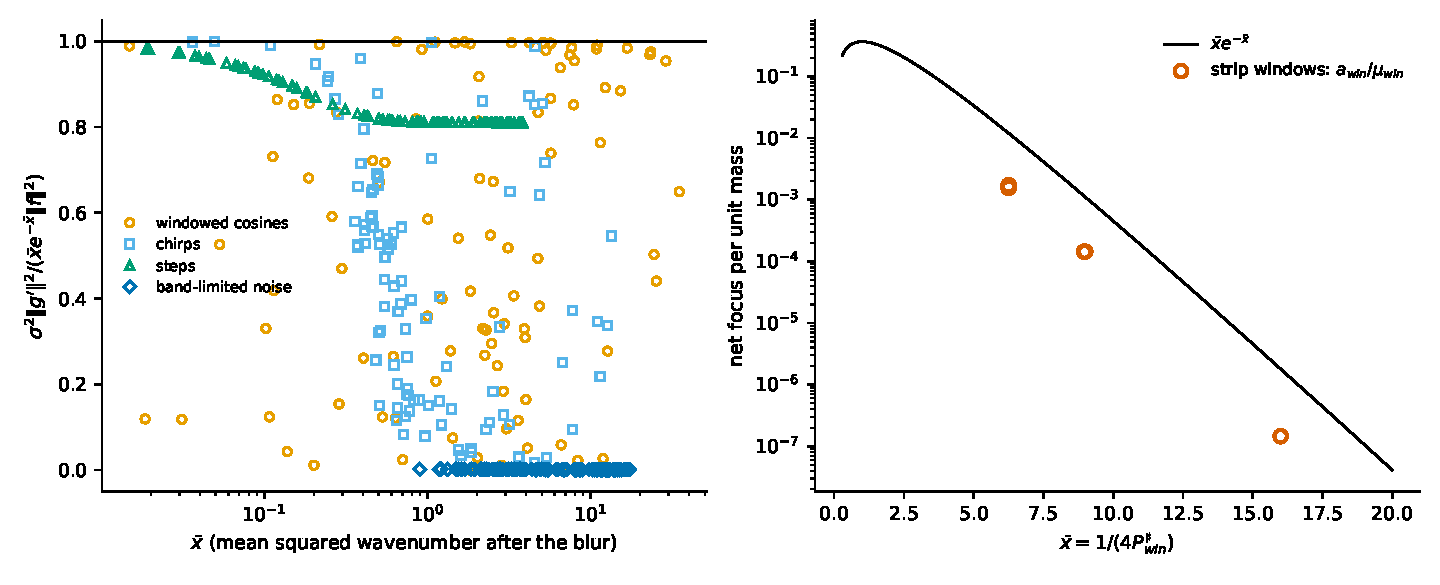
\includegraphics[width=0.85\textwidth]{figures/fig4_lemma.pdf}
\caption{(a) Lemma~\ref{lem:smoothing1d} on random one-dimensional structures: the ratio of the two sides of Eq.~\eqref{eq:smoothing1d} never exceeds one, and approaches one for a single wavenumber. (b) Sharpness per unit mass of the windows of the strips against $\bar x e^{-\bar x}$, with $\bar x$ taken from the window's spread (observed, not proved).}
\label{fig:lemma}
\end{figure*}

In the plane we apply the same argument to the part of the density that varies along the stable direction, with one refinement: we split the blur into two parts, use the first to remove fine structure and keep the second to compare norms. The confinement of the state then provides the floor.

\begin{lemma}[Split smoothing--uncertainty]
\label{lem:split}
Under (H1), for every $t \in (0,1)$,
\begin{equation}
\xb(\varrho) \leq \frac{1}{t}\Big[2\ln\frac1\sigma + \ln\frac{8(\pi^2 + \sigma^2/2)}{e\,t(1-t)}\Big].
\label{eq:split}
\end{equation}
Without (H1) the same holds with $\pi^2 + \sigma^2/2$ replaced by the state's own $\E_Q[y_z^2]$.
\end{lemma}

The proof (Appendix~\ref{app:split}) has four steps. Write $\varrho$ as a blur of variance $t\sigma^2$ of the partly blurred state $\rho * N(0,(1-t)\sigma^2)$. (i)~Jensen's inequality, as in Lemma~\ref{lem:smoothing1d}, shows that the second blur reduces $\|\partial_w\varrho\|^2$ by at least $e^{-t\xb}$. (ii)~Since $\rho \geq 0$, the partly blurred state has an $L^2$ norm at most $(1-t)^{-1/2}$ times that of $\varrho$. (iii)~On each line $v = \text{const}$, the Heisenberg inequality in $w$ bounds $\|\partial_w\varrho\|^2$ from below by $\|\varrho\|^2/(8\E_Q[y_z^2])$. (iv)~The square $\varrho^2$ is itself a blur, of variance $\sigma^2/2$, of the midpoints of pairs of points of the state; this is why (H1) bounds $\E_Q[y_z^2]$. In observer language: a state confined near the top cannot be flat along the stable direction, and the blur erases fine structure faster than that confinement can pay for.

\subsection{The logarithmic law}

To pass from $\varrho$ to $\sqrt\varrho$, which enters Corollary~\ref{cor:regular}, we need the ratio
\begin{equation}
K_\Lambda = \frac{\xb(\sqrt\varrho)}{\xb(\varrho)} .
\end{equation}
It compares the fineness of $\sqrt\varrho$, which weights structure by its mass, with that of $\varrho$, which weights it in $L^2$. It equals $1/2$ for a Gaussian state.

\begin{theorem}[Logarithmic lower bound]
\label{thm:log}
Under (H1) and $K_\Lambda \leq K_1$, for every $t \in (0,1)$,
\begin{gather}
g \geq \Pi\;\frac{\sqrt t}{2\pi\sqrt{K_1}}\;\frac{1}{\sqrt{\ln(1/\sigma) + C_t}}, \label{eq:log}\\
C_t = \frac12\ln\frac{8(\pi^2 + \sigma^2/2)}{e\,t(1-t)} . \nonumber
\end{gather}
At $t = 1/2$, $c = 0.1125/\sqrt{K_1}$ and $C_t \leq 2.40$ for $\sigma \leq 1$. Choosing $t \to 1$ slowly as $\sigma \to 0$ gives $c \to 1/(2\pi\sqrt{K_1})$, with $C$ growing like $\frac12\ln\ln(1/\sigma)$.
\end{theorem}

\begin{proof}
By Corollary~\ref{cor:regular}, $g \geq \Pi\sqrt2/(\pi\sqrt\Lambda)$ with $\Lambda = 4K_\Lambda\xb(\varrho) \leq 4K_1\xb(\varrho)$, and Lemma~\ref{lem:split} gives $\xb(\varrho) \leq 2(\ln(1/\sigma) + C_t)/t$.
\end{proof}

The theorem says that the blur allows fine structure only up to $\xb \approx 2\ln(1/\sigma)$: below that scale it erases more structure along the stable direction than the confined state can afford to lose. Since the gap is at least of order $1/\sqrt{\xb}$, it can shrink at most like $1/\sqrt{\ln(1/\sigma)}$.

Each step of the chain was checked numerically on 415 states (Gaussian mixtures, stored and adversarial, localised ripples, two clusters, and the strip optima from $\sigma = 10^{-2}$ to $10^{-96}$) and two values of $t$, with no violation. On the strips $K_\Lambda \leq 0.99$, so the theorem applies to them with $K_1 = 1$. Figure~\ref{fig:staircase} compares it with the strips: the numerical minimum lies above the bound at every $\sigma$, by a factor between 33 at $\sigma = 10^{-2}$ and 6.9 at $\sigma = 10^{-96}$. Two steps account for most of the remaining factor: the bound $1 - \cos m \geq 2m^2/\pi^2$, which loses $\pi/\sqrt2 \approx 2.2$ near the top, and the uniform estimate $2\ln(1/\sigma)$ of $\xb$, which is larger than the strips' own $\xb$ because the strips vary along $w$ on the scale $\sqrt\sigma$ rather than $\sigma$. The Heisenberg and Jensen steps become nearly tight on the strips.

\begin{figure}[t]
\centering
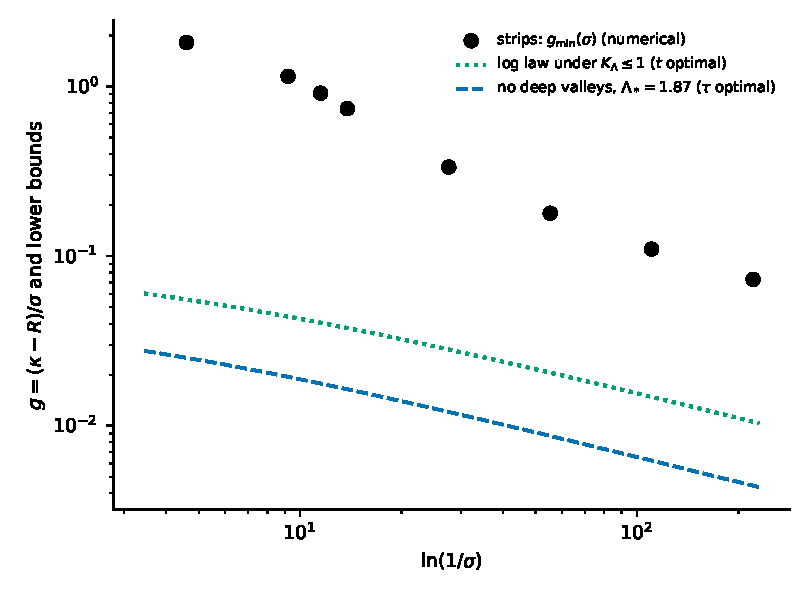
\includegraphics[width=\columnwidth]{figures/fig3_staircase.pdf}
\caption{Lower bounds on $g = (\kappa - R)/\sigma$ against the strips' numerical minimum $g_{\min}(\sigma)$ (dots), with the prefactor $\Pi$ set to one. Dotted: Theorem~\ref{thm:log} with $K_1 = 1$, which covers the strips, and $t$ chosen optimally at each $\sigma$. Dashed: Proposition~\ref{prop:novalley} with the strips' $\Lambda_* = 1.87$, which needs no ratio condition. Both decrease like $1/\sqrt{\ln(1/\sigma)}$, as the strips do.}
\label{fig:staircase}
\end{figure}

\subsection{The ratio $K_\Lambda$}

The ratio $K_\Lambda$ is checkable state by state, and it was small on every family with a small gap: $0.46$--$0.99$ on the strips, $0.69$--$0.78$ on localised ripples, $0.5$ on two clusters, $0.64$ on the hourglass mixture of Ref.~\cite{namba2026gap}, and at most $0.68$ over 36 adversarial maximisations restricted to states with $\sqrt{P_w} \leq 1$. It has, however, no universal bound. For a product state $\rho_1(v)\rho_2(w)$ one finds exactly $K_\Lambda = J_v\|\varrho_v\|^2/(4\|\varrho_v'\|^2)$, where $\varrho_v$ is the blurred first factor and $J_v$ its Fisher information. A wide factor plus a narrow bump of low density gives $K_\Lambda = 0.7$, $1.7$, $5.3$, $23$ and $43$ at $\sigma = 10^{-2}, \dots, 10^{-12}$. These states have large gaps ($\sqrt{P_w}$ between $2.2$ and $10^6$), so they are not counterexamples to the logarithmic law. They show a limit of the proof: $\sqrt\varrho$ sees fine structure in regions of low density that $\varrho$ hardly sees, while such structure cannot support the sharpness near the top that a small gap needs. Section~\ref{sec:removing} removes the ratio condition for broad classes of states by a different route.

\section{Ripple strips: numerical evidence that the uniform gap fails}
\label{sec:strips}

\subsection{The family}

Corollary~\ref{cor:regular} says where to look for small gaps: at states with fine structure along the unstable direction that varies along the stable direction. The simplest such states are ripple strips,
\begin{equation}
\rho(v,w) = N(v;0,L_v^2)\,N(w;0,L_w^2)\,\Big[1 + c\,e^{-w^2/2\ell^2}\cos\frac{k_0 v}{\sigma}\Big],
\label{eq:strip}
\end{equation}
a Gaussian background of widths $L_v$ and $L_w$ carrying a ripple of wavenumber $k_0/\sigma$ along $v$, confined to a window of width $\ell$ along $w$, with amplitude $0 \leq c \leq 1$. We write $\ell = \lambda\sqrt\sigma$ and $L_w = M\ell$. The free parameters are $k_0$, $\lambda$, $M$, $L_v$ and $c$, and every state below satisfies $\Upsilon \leq 1/2$.

In observer language, the ripple makes the state sharp along the unstable direction, but only inside the window, close to the line through the top; the long background along $w$ supplies the small information along the stable direction that the gap formula~\eqref{eq:formula} asks for. Both the blurred density and the posterior moments of Eq.~\eqref{eq:strip} are available in closed form, since every term is a Gaussian, with a complex mean for the ripple (Appendix~\ref{app:methods}).

\subsection{The gap tends to $1/(2k_0)$}

\begin{observation}
\label{obs:limit}
In the limit $\sigma\to 0$, minimised over $\lambda$, $M$ and $L_v$ at fixed $k_0$, the strips reach
\begin{equation}
g \to \frac{1}{2k_0}
\end{equation}
within $0.1\%$ for $k_0 = 1.5, 2, 2.5, 3, 4, 5, 6$ (Fig.~\ref{fig:strip}). In this limit the inequality of arithmetic and geometric means in Theorem~\ref{thm:direct} becomes an equality and $\varepsilon \to 0$.
\end{observation}

\begin{figure}[t]
\centering
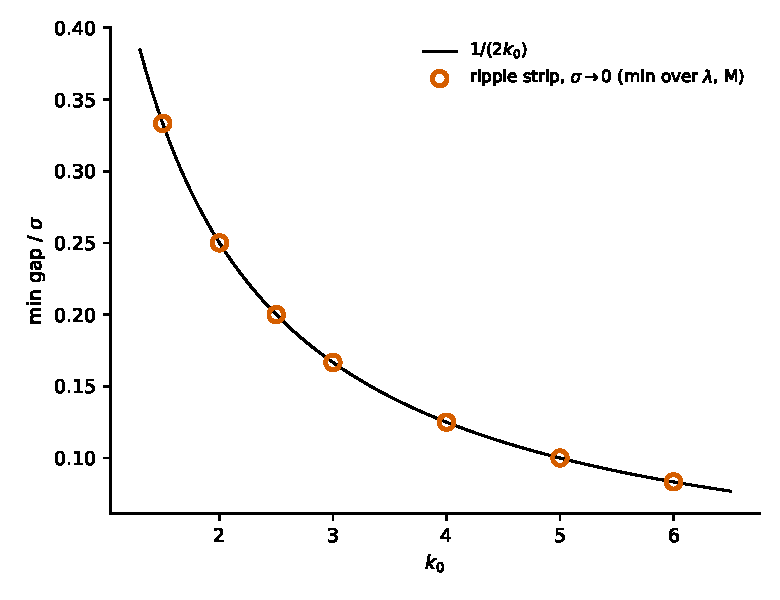
\includegraphics[width=0.85\columnwidth]{figures/fig1_strip_limit.pdf}
\caption{Minimum gap of the strips in the limit $\sigma \to 0$ (computed at $\sigma = 10^{-80}$), at fixed ripple wavenumber $k_0$ and minimised over the other parameters. The line is $1/(2k_0)$.}
\label{fig:strip}
\end{figure}

So the gap in units of $\sigma$ can be made as small as one likes, provided $k_0$ can be made large. The price is the one of Lemma~\ref{lem:smoothing1d}. The blur reduces the ripple's contribution to the sharpness by $e^{-k_0^2}$, so that the window becomes very faint, and the background must become long, $M \gtrsim e^{k_0^2}$, to keep the information along $w$ smaller still. A long background in turn feels the nonlinearity of the pendulum. Balancing these costs at fixed $\sigma$ allows $k_0$ to grow only like $\sqrt{\ln(1/\sigma)}$. At $\sigma = 10^{-80}$, for instance, $k_0 = 7$ is already too expensive: its best gap is $3.28\,\sigma$.

\subsection{The smallest gap at a given resolution}

\begin{observation}
\label{obs:gmin}
The minimum of $g$ over the strips at a given $\sigma$, $g_{\min}(\sigma)$, is listed in Table~\ref{tab:gmin} and shown in Fig.~\ref{fig:gmin}. It decreases to zero. For $\sigma \leq 10^{-24}$ it follows
\begin{equation}
g_{\min}(\sigma) \approx \frac{A}{\sqrt{\ln(1/\sigma) - B}}, \qquad A = 1.02,\quad B = 23.4,
\label{eq:fit}
\end{equation}
with a largest relative residual of $1.1\%$, and the local exponent $d\ln g_{\min}/d\ln\ln(1/\sigma)$ decreases in magnitude from $-1.14$ to $-0.60$ towards $-1/2$. The strips go below the Gaussian-mixture minimum $0.884$ only for $\sigma \lesssim 7.1\times 10^{-6}$.
\end{observation}

\begin{table}[t]
\caption{Smallest gap $g_{\min}(\sigma) = \min (\kappa - R)/\sigma$ over the strips~\eqref{eq:strip}, and the ripple wavenumber $k_0$ of the optimum.}
\label{tab:gmin}
\begin{ruledtabular}
\begin{tabular}{lcc}
$\sigma$ & $g_{\min}$ & $k_0$ \\
\hline
$10^{-2}$ & 1.818 & 0.98 \\
$10^{-4}$ & 1.149 & 1.08 \\
$10^{-5}$ & 0.914 & 1.12 \\
$10^{-6}$ & 0.740 & 1.23 \\
$10^{-12}$ & 0.335 & 1.85 \\
$10^{-24}$ & 0.179 & 3.00 \\
$10^{-48}$ & 0.110 & 4.66 \\
$10^{-96}$ & 0.073 & 6.96 \\
\end{tabular}
\end{ruledtabular}
\end{table}

\begin{figure}[t]
\centering
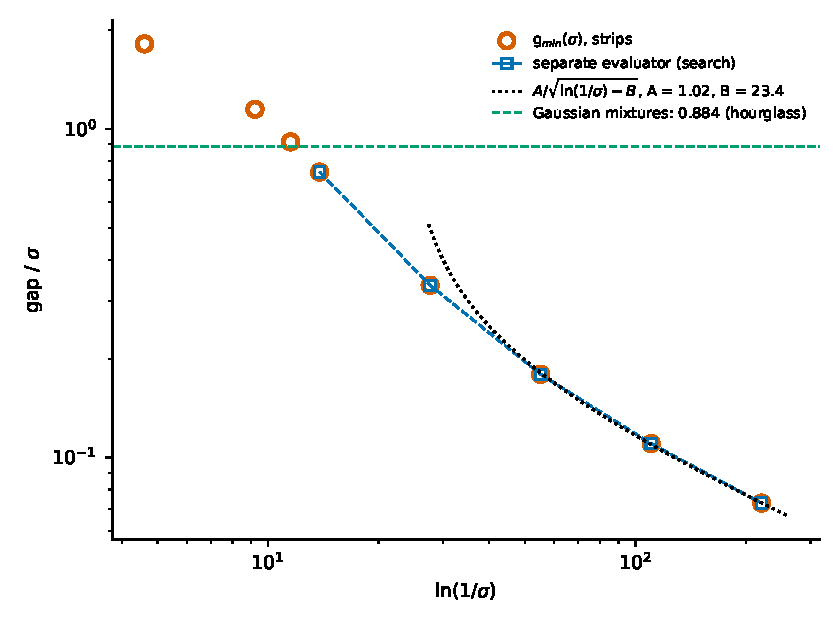
\includegraphics[width=0.9\columnwidth]{figures/fig2_gmin.pdf}
\caption{Smallest gap of the strips at a given $\sigma$ (circles: main evaluators; squares: a separate evaluator used in the search), the fit~\eqref{eq:fit} (dotted), and the minimum over Gaussian mixtures with up to 32 components (dashed).}
\label{fig:gmin}
\end{figure}

The coefficient $A \approx 1$ agrees with the balance above: $g \approx 1/(2k_0)$ with $k_0^2 \approx \ln(1/\sigma)/4$ minus slowly growing corrections. It also agrees with the proved side. On the strip optima $\xb(\sqrt\varrho)$ approaches $k_0^2$ as $\sigma\to 0$ (at $\sigma = 10^{-96}$, $\xb(\varrho) = 48.2$ and $K_\Lambda = 0.99$, against $k_0^2 = 48.4$), so that Corollary~\ref{cor:regular} gives $g \gtrsim 1/(\pi\sqrt2\,k_0)$. This is below the observed $1/(2k_0)$ by the factor $\pi/\sqrt2 \approx 2.2$ lost in Eq.~\eqref{eq:PwP}, the dominant looseness of Theorem~\ref{thm:log} on the strips.

We also searched beyond the single strip, at $\sigma = 10^{-12}$ and $10^{-24}$: superpositions of the wavenumbers $k$ and $2k$, three interfering windows with free phases, windows with different $k_0$ side by side along $w$, and the first three harmonics. None went below the single strip; the best members were higher by $0.07\%$ to $1.6\%$, and the optimiser removed the extra components. This agrees with Lemma~\ref{lem:smoothing1d}, in which equality requires a single wavenumber, but the search was local.

\subsection{How the numbers were checked}

The gap of the strips is a small difference of large quantities. At $\sigma = 10^{-24}$, for instance, the numerator of Eq.~\eqref{eq:formula} is of order $10^{-34}$ while its building blocks are many orders of magnitude larger, and a direct evaluation fails; an early version of this study was misled by a rounding artefact in one of the building blocks (Appendix~\ref{app:methods}). Every value in Table~\ref{tab:gmin} was therefore computed by at least two evaluators that share no code for the states, the pointwise fields or the integration, including a full two-dimensional grid where feasible and a 320-digit pointwise check. In addition, the values at $\sigma = 10^{-4}$, $10^{-6}$, $10^{-12}$, $10^{-24}$ and $10^{-48}$ were reproduced to ten digits or better by an evaluator written separately from the closed-form expressions of Appendix~\ref{app:methods}, whose formulas were in turn checked pointwise against direct two-dimensional quadrature of the posterior; an optimisation with that evaluator from unrelated starting points found the same optima at $\sigma = 10^{-12}$ and $10^{-24}$.

\section{Removing the ratio condition: unconditional theorems}
\label{sec:removing}

\subsection{What has to be shown}

Corollary~\ref{cor:regular} needs a bound on $\Lambda = 4\xb(\sqrt\varrho)$ itself. Theorem~\ref{thm:log} obtained one through $\xb(\varrho)$ and the ratio $K_\Lambda$. A direct route needs only the following form, in which the information along the stable direction plays the role of the scale.

\begin{proposition}[Target inequality]
\label{prop:target}
Suppose that $\Lambda \leq A + B\ln\big(1/(\sigma^2 J_{ww})\big)$ for a state satisfying (H2). Then
\begin{gather}
g \geq \Pi\,\frac{c}{\sqrt{\ln(1/\sigma) + C}}, \qquad c = \frac{1}{\pi\sqrt B}, \label{eq:target}\\
C = \frac12\ln\big(2(\pi^2 + \sigma^2)\big) + \frac{A}{2B}. \nonumber
\end{gather}
\end{proposition}

\begin{proof}
Insert Eq.~\eqref{eq:CR} into the hypothesis and the result into Corollary~\ref{cor:regular}.
\end{proof}

By Lemma~\ref{lem:fisher}(b) below, $\Lambda \leq 2 + 8tR$, where $tR$ is the rate at which the information along the stable direction is lost under further blurring (Eq.~\eqref{eq:Rdef}). The theorems below prove the hypothesis of Proposition~\ref{prop:target} for their classes in the stronger form
\begin{equation}
tR \leq A' + B'\ln\frac{1}{tJ_{ww}},
\label{eq:T2}
\end{equation}
which gives $B = 8B'$ and $A = 2 + 8A'$. For general states we conjecture the law itself:

\begin{conjecture}[Logarithmic law for all states]
\label{conj:general}
There are constants $c > 0$ and $C$ such that every state satisfying (H1) and (H2) obeys $g \geq \Pi\,c/\sqrt{\ln(1/\sigma) + C}$.
\end{conjecture}

We state the conjecture for the gap rather than for Eq.~\eqref{eq:T2}, because Eq.~\eqref{eq:T2} with universal constants is not true for every state. In work to be reported separately we find states in which hidden sources of alternating sign sit in a deep valley between long lines along $w$; for them $tR/\ln(1/(tJ_{ww}))$ grows without bound as the number of sources grows (numerical results and a leading-order analysis). Such states need lines whose length is exponential in the depth of the valley, so (H2) limits the effect, and they do not by themselves contradict Conjecture~\ref{conj:general}.

\subsection{The Fisher form and the heat flow}

Write $t$ for the blur variance and follow the state along the heat flow $\partial_t\varrho = \frac12\Delta\varrho$, which is the blur growing from $t = 0$ to $t = \sigma^2$. Define the rate at which the information along the stable direction is lost,
\begin{equation}
R(t) = -\frac{d\ln J_{ww}}{dt} .
\label{eq:Rdef}
\end{equation}

\begin{lemma}[Fisher form]
\label{lem:fisher}
For every state, (a)~$\Lambda \leq 2 + 8t\,\E[H_{vw}^2]/J_{ww}$; (b)~$dJ_{ww}/dt = -\E[H_{vw}^2 + H_{ww}^2]$, so that $tR = t\,\E[H_{vw}^2 + H_{ww}^2]/J_{ww}$ and $\Lambda \leq 2 + 8tR$; (c)~with $u = s_w$ and $L = \Delta + s\cdot\nabla$,
\begin{equation}
J_{ww}R' = -\E[(Lu + Ru)^2] - \E[(H^3)_{ww}] .
\label{eq:gamma2}
\end{equation}
\end{lemma}

Part (a) follows from two integrations by parts and the bound $H_{vv} \leq 1/t$, which holds because the posterior covariance $t I - t^2 H$ is positive semidefinite; (b) is a directional de~Bruijn identity; (c) is the Bochner, or $\Gamma_2$, identity of the operator $L$~\cite{bakry2014} applied to $u$. The proofs are in Appendix~\ref{app:fisher}. The first term of Eq.~\eqref{eq:gamma2} is never positive. The second can be positive only where $H$ has a negative eigenvalue, that is, where the blurred density is log-convex in some direction: in the valleys between peaks. In particular, for a log-concave state $H \succeq 0$, so $R$ never increases and $J_{ww}$ is log-convex along the heat flow, a directional counterpart of the concavity of $1/I$ along the heat flow for log-concave densities~\cite{toscani2015}. For multimodal states $R$ can increase; for two clusters we found $R(\sigma^2/4)/R(\sigma^2) = 0.70$.

The heat flow converts a bound on the growth of $R$ into the target inequality.

\begin{lemma}[Integration along the heat flow]
\label{lem:integration}
If $t^2R'(t) \leq A_1\,tR(t) + \kappa_1$ for all $t \in [\tau\sigma^2, \sigma^2]$, with constants $A_1, \kappa_1 \geq 0$ and $\tau \in (0,1)$, then
\begin{equation}
\Lambda \leq 2 + 8c_0 + B\Big[\ln\frac1\tau + \ln\frac{1}{\sigma^2 J_{ww}}\Big], \qquad B = \frac{8(1 + A_1)}{1 - \tau^{1+A_1}},
\end{equation}
with $c_0 = \kappa_1\big[\ln(1/\tau)/(1 - \tau^{1+A_1}) - 1/(1 + A_1)\big]$.
\end{lemma}

\begin{proof}
The hypothesis gives $d(s^{-A_1}R)/ds \leq \kappa_1 s^{-A_1-2}$, so that $R(s) \geq (s/\sigma^2)^{A_1}R(\sigma^2) - \kappa_1\big(1/s - s^{A_1}/\sigma^{2+2A_1}\big)/(1+A_1)$ for $s \leq \sigma^2$. Integrating over $[\tau\sigma^2, \sigma^2]$ and using $\int R = \ln\big(J_{ww}(\tau\sigma^2)/J_{ww}(\sigma^2)\big)$ and $J_{ww}(\tau\sigma^2) \leq 1/(\tau\sigma^2)$, the Fisher information of a blur of variance $\tau\sigma^2$, bounds $\sigma^2 R(\sigma^2)$. Lemma~\ref{lem:fisher}(b) then bounds $\Lambda$.
\end{proof}

So the question becomes whether the valleys, the only source of growth of $R$ in Eq.~\eqref{eq:gamma2}, can be controlled.

\subsection{Deep valleys cost Fisher information}

On a line, the blurred density is the Gaussian blur of a positive measure. Let $c(y)$ be the posterior variance at $y$ in units of $t$, so that $c - 1 = -t\,\partial^2\ln\varrho$; a valley is a point with $c > 1$, and a deep valley one with $c \geq 1 + \eta$. In units $t = 1$:

\begin{lemma}[A valley is a dip]
\label{lem:dip}
$\ln\varrho(y+u) + \ln\varrho(y-u) - 2\ln\varrho(y) \geq \ln\cosh\big(u\sqrt{2c(y)}\big) - u^2$ for all $u$.
\end{lemma}

\begin{proof}
$\varrho(y\pm u) = \varrho(y)e^{-u^2/2}\E_y[e^{\pm u(X - y)}]$, with $\E_y$ the posterior at $y$. The product of the two is $\varrho(y)^2e^{-u^2}\E[\cosh(u(X - X'))]$ for two independent posterior copies, and $x \mapsto \cosh(u\sqrt x)$ is convex, so Jensen's inequality gives $\E[\cosh(u|X - X'|)] \geq \cosh(u\sqrt{2c})$.
\end{proof}

For $c$ well above one the right side is positive: the valley point lies at the bottom of a dip of depth about $u\sqrt{2c} - u^2$. Climbing out of a dip requires score. If $\varrho(b) \geq \varrho(a)e^{\Delta}$ with $\Delta \geq 0$, then $\int_a^b \varrho\,s^2 = 4\int_a^b (\sqrt\varrho\,')^2 \geq 4\varrho(a)(e^{\Delta/2} - 1)^2/(b - a)$ by the Cauchy--Schwarz inequality. Applying this on both sides of the dip, with the convexity of $x \mapsto (e^{x/2}-1)_+^2$, gives $\varrho(y) \leq u\big(8(e^{D/4} - 1)^2\big)^{-1}\int_{|y'-y| \leq u}\varrho\,s^2$, where $D$ is the right side of Lemma~\ref{lem:dip}. Integrating over the valley points, exchanging the integrals and choosing $u$ for each range of $c$ gives:

\begin{theorem}[Valleys cost Fisher information]
\label{thm:valley}
For every state on a line and every $\eta > 0$,
\begin{equation}
\E\big[(c - 1)^3\,\mathbf{1}\{c \geq 1 + \eta\}\big] \leq \kappa_\eta\, t J,
\end{equation}
where $J$ is the Fisher information and $\kappa_\eta$ is an explicit constant; $\kappa_{0.1} = 267$.
\end{theorem}

The constant is loose: the largest value of the left side divided by $tJ$ that we found is about $3$. In observer language: where the observer is very unsure from which part of the state a point came, the density has a dip, and the slopes of the dip are score, that is, information.

\begin{theorem}[Product states]
\label{thm:product}
Let $\rho(x) = \rho_1(f\cdot x)\rho_2(l\cdot x)$ for an orthonormal pair $(f, l)$ at any angle, including states concentrated on a line, and let (H2) hold. Then $t^2R' \leq \eta\,tR + \kappa_\eta$ for every $t$ and $\eta > 0$, and the logarithmic law~\eqref{eq:target} holds without any ratio condition, with $B = 8(1+\eta)/(1-\tau^{1+\eta})$ for any $\tau \in (0,1)$. For $\eta = 0.1$ and $\tau = 1/4$, $c = 0.0949$ and $C = 84$ ($\sigma \leq 1$).
\end{theorem}

\begin{proof}
The blur preserves the product form, and $H$ is diagonal in $(f, l)$. With $a = (e_w\cdot f)^2$, $-(tH)^3_{ww} = a(c_f - 1)^3 + (1-a)(c_l - 1)^3$ and $J_{ww} = aJ_{ff} + (1-a)J_{ll}$, where $c_f$, $c_l$ are the posterior variances of the two factors. The part with $c < 1 + \eta$ is at most $\eta\,(tH)^2_{ww}$, and Theorem~\ref{thm:valley} for each factor bounds the rest by $\kappa_\eta tJ_{ww}$. Dropping the first term of Eq.~\eqref{eq:gamma2} gives $t^2R' \leq \E[-(tH)^3_{ww}]/(tJ_{ww}) \leq \eta\,tR + \kappa_\eta$. Lemma~\ref{lem:integration} and Proposition~\ref{prop:target} complete the proof.
\end{proof}

The large $C$ reflects only the loose $\kappa_\eta$; the coefficient $c$ does not depend on it.

\subsection{States without deep valleys, and the strips}
\label{sec:novalley}

In the plane the same mechanism works whenever the valleys stay shallow.

\begin{proposition}[No deep valleys]
\label{prop:novalley}
Suppose that (H2) holds and that for some $\tau \in (0,1)$ and $\Lambda_* \geq 0$ the posterior covariance satisfies $\Cov(X\mid y) \preceq (1 + \Lambda_*)\,t\,I$ for every $y$ and every blur $t \in [\tau\sigma^2, \sigma^2]$. Then $t^2R' \leq \Lambda_*\,tR$ on that window, and the logarithmic law~\eqref{eq:target} holds with $B = 8(1+\Lambda_*)/(1 - \tau^{1+\Lambda_*})$ and $A = 2 + B\ln(1/\tau)$.
\end{proposition}

\begin{proof}
The hypothesis says that every eigenvalue $\lambda_i$ of $-tH$ is at most $\Lambda_*$. With $a_i = (e_w\cdot f_i)^2$ for the eigenvectors $f_i$, $-(tH)^3_{ww} = \sum_i\lambda_i^3 a_i \leq \Lambda_*\sum_i\lambda_i^2a_i = \Lambda_*(tH)^2_{ww}$, since the terms with $\lambda_i \leq 0$ are not positive. Equation~\eqref{eq:gamma2} gives $t^2R' \leq \Lambda_*\,tR$, and Lemma~\ref{lem:integration} with $\kappa_1 = 0$ and Proposition~\ref{prop:target} complete the proof.
\end{proof}

\begin{observation}
\label{obs:novalley}
On the eight strip optima of Table~\ref{tab:gmin}, the largest eigenvalue of $-tH$ over all points and over 25 blurs $t \in [\sigma^2/4, \sigma^2]$ is $\Lambda_* = 1.8745$, at $\sigma = 10^{-2}$ and $t = \sigma^2/4$ (Fig.~\ref{fig:valleys}a). It decreases with $t$ on every strip, and its maximum over the window falls from $1.87$ at $\sigma = 10^{-2}$ to $0.38$ at $10^{-48}$ and $0.03$ at $10^{-96}$. Proposition~\ref{prop:novalley} then gives $c = 0.0658$ and $C = 2.28$ for the strips ($\tau = 1/4$, $\sigma \leq 1$).
\end{observation}

The values at $\sigma = 10^{-2}$ ($1.874$, $1.756$ and $1.537$ at $t = \sigma^2/4$, $\sigma^2/2$ and $\sigma^2$) were reproduced by an independent evaluation on a two-dimensional Fourier grid. The verification is a dense-grid evaluation, not interval arithmetic. In observer language, the strips never make the observer much more unsure than the blur itself: their fineness consists of shallow ripples, not valleys. On the strips Theorem~\ref{thm:log} with $K_1 = 1$ also applies, with a better constant (Fig.~\ref{fig:staircase}). The point of Proposition~\ref{prop:novalley} is that its hypothesis concerns valleys, the mechanism that Eq.~\eqref{eq:gamma2} identifies, rather than a ratio of norms.

\begin{figure}[t]
\centering
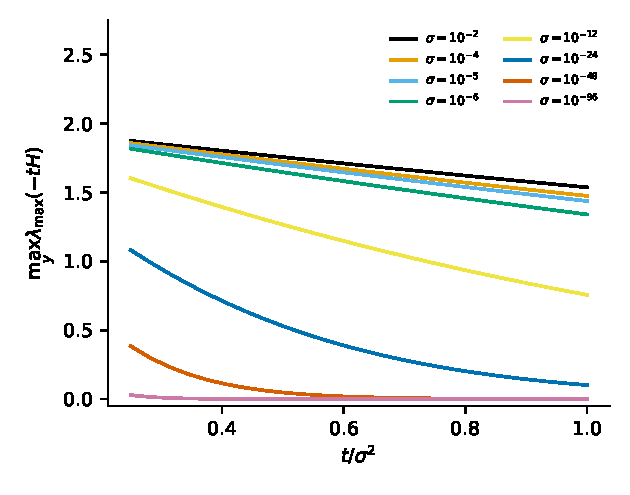
\includegraphics[width=0.95\columnwidth]{figures/fig5_valleys.pdf}
\caption{The strips have no deep valleys: largest eigenvalue of $-tH$ over all points, against the blur $t$ in the window of Proposition~\ref{prop:novalley}, for the eight strip optima. The values stay below $1.88$ and fall towards zero as $\sigma$ decreases.}
\label{fig:valleys}
\end{figure}

\subsection{What is now unconditional}

Putting the pieces together, the logarithmic law~\eqref{eq:target} holds with no ratio condition, under (H2) alone, for
\begin{itemize}
\item every product state $\rho_1(f\cdot x)\rho_2(l\cdot x)$, at any angle, including states concentrated on a line (Theorem~\ref{thm:product});
\item every state whose posterior covariance stays below $(1+\Lambda_*)$ times the blur on the window $[\tau\sigma^2, \sigma^2]$ (Proposition~\ref{prop:novalley}); the strips, the states that realise the smallest gaps we found, are in this class with $\Lambda_* = 1.87$ (Numerical result~\ref{obs:novalley}).
\end{itemize}
In both cases the mechanism is the same, and it is the one the observer would guess. Fine structure is what lets a state come close to $\kappa$, and the blur takes it away exponentially. The only way the blur can strip information faster is through valleys, places where the observer cannot tell from which part of the state a point came; and a valley is a dip whose slopes are paid for in information. The strips, which come closest to the edge, never pay that price: their fineness is all in shallow ripples.

What remains is Conjecture~\ref{conj:general} for states that do have deep valleys. Following the blur as it grows, the route used here, is not enough for every such state, and the confinement (H2) has to enter the argument (Sec.~\ref{sec:discussion}).

\section{Discussion}
\label{sec:discussion}

\subsection{What is established}

The answer to the uniform-gap question at the top of the pendulum is negative: no constant $c > 0$ independent of $\sigma$ gives $\kappa - R \geq c\sigma$ for all states. The counterexamples are numerical, but every number was confirmed by evaluations that share no code, and their behaviour, $g \to 1/(2k_0)$ with $k_0$ limited to $\sqrt{\ln(1/\sigma)}$ by the cost of the blur, is explained by the same mechanism that the proofs use.

What survives is a logarithmic law, and both of its sides have the same form. The strips show that $g_{\min}(\sigma)$ can decrease like $1/\sqrt{\ln(1/\sigma)}$. The lower bounds show that it cannot decrease faster: for every state with a bounded ratio $K_\Lambda$ (Theorem~\ref{thm:log}), and without any ratio condition for product states in any orientation (Theorem~\ref{thm:product}) and for states without deep valleys (Proposition~\ref{prop:novalley}), the class that contains the strips. The states that come closest to the edge are therefore covered by a theorem without any ratio condition, whose one hypothesis, the absence of deep valleys, we verified on them numerically. On the strips the best proved constant is below the numerical one by a factor of about 7 at the smallest $\sigma$, and most of the factor comes from two identified steps. This is the familiar structure of a limit theorem with a matching construction, here with the limit proved for broad classes and the construction established numerically.

The proofs also isolate what controls the gap: the single number $\xb$, the fineness of the structure along the unstable direction after the blur. In observer language, the gap is a tug of war between the information along the stable direction and the nonlinearity felt where the state is sharp (Theorem~\ref{thm:direct}). Fine structure lets a state be sharp close to the top, which is what a small gap requires, but the blur erases fine structure exponentially (Lemmas~\ref{lem:smoothing1d} and~\ref{lem:split}), and a state confined near the top cannot afford to lose its last structure along the stable direction. The result is a ceiling $\xb \lesssim 2\ln(1/\sigma)$ and a gap of order $\sigma/\sqrt{\ln(1/\sigma)}$. The second route adds a second picture: following the blur as it grows, the only thing that can make the observer lose information faster is a valley, a place where the observer cannot tell from which part of the state a point came, and such a valley sits in a dip whose slopes carry information (Theorem~\ref{thm:valley}).

The effect matters only at very fine resolution. Gaussian mixtures with up to 32 components stayed above $0.884\,\sigma$, the best Gaussian state tends to $\sigma$~\cite{namba2026gap}, and the strips beat the mixtures only below $\sigma \approx 7\times 10^{-6}$. At such resolutions the factor $1/\sqrt{\ln(1/\sigma)}$ is close to $0.3$. For practical purposes the resolution gap of Refs.~\cite{namba2026gap,namba2026many} stands as a proportionality to $\sigma$; as a mathematical statement it carries a logarithm.

\subsection{Open problems}

\begin{enumerate}
\item \emph{The logarithmic law for all states.} No counterexample to Conjecture~\ref{conj:general} is known. The intermediate inequality~\eqref{eq:T2} holds on all 1778 stored pairs of a state and a blur, with $tR \leq \ln(1/(tJ_{ww})) + 6.54$, but not with universal constants for every state: hidden sources of alternating sign in the valley between very long lines defeat it (Sec.~\ref{sec:removing}). A proof for general states must therefore use the confinement (H2), which caps $\ln(1/(\sigma^2J_{ww}))$ at $2\ln(1/\sigma) + O(1)$ through Eq.~\eqref{eq:CR}, and not only the structure of the blur. We shall report on this separately.
\item \emph{The remainders.} $\varepsilon$, $\varepsilon_m$ and $\varepsilon_\pi$ are explicit and were small on every focused state ($|\varepsilon| \leq 0.004$, $\varepsilon_m \leq 0.11$), but state-independent bounds on $\varepsilon$ are not known.
\item \emph{The strips analytically.} The limit $g \to 1/(2k_0)$, the law~\eqref{eq:fit} and the absence of deep valleys are numerical. An asymptotic analysis of Eq.~\eqref{eq:strip} would turn the construction side into a theorem.
\item \emph{Beyond the pendulum.} The mechanism uses only the Gaussian blur, the uncertainty principle and the confinement of the state near a hyperbolic point. We expect a logarithmic law at the hyperbolic points of other flows and in many degrees of freedom, with the matrix formula of Ref.~\cite{namba2026many} in place of the pendulum's constant, but this has not been checked.
\end{enumerate}

\subsection{Relation to other work}

Finite-resolution entropies are used as diagnostics of chaos, where the growth rate of a coarse-grained entropy tracks the Lyapunov exponent~\cite{kannan2026}. Those studies fix the resolution; here the resolution widens in time, and the question is the margin by which the onset of entropy growth stays below the stretching rate. The heat-flow part of Sec.~\ref{sec:removing} belongs to the study of Fisher information along the heat flow, where de~Bruijn's identity and the $\Gamma_2$ calculus are standard tools~\cite{cover2006,bakry2014} and convexity properties are known for log-concave densities~\cite{toscani2015}; the directional and multimodal setting here, and the role of valleys, appear to be outside those results. For phase-space diffusion models~\cite{dockhorn2022,namba2026threshold,namba2026learned}, the present result says that data with fine structure can narrow the band between the two thresholds $R$ and $\kappa$ found in Ref.~\cite{namba2026learned}, and, for the classes covered by the theorems, only logarithmically in the noise level.


\appendix
\section{Proof of Theorem~\ref{thm:direct} and the remainder}
\label{app:direct}

\paragraph*{Identity~\eqref{eq:identity}.}
Write $h(z) = z - \sin z$. In Eq.~\eqref{eq:Ncov}, expand $h(X_z)$ around the posterior mean $m_z$: the first-order term gives $\Cov(X_p, X_z\mid y)\,h'(m_z) = -\sigma^4 H_{pz}\,\phi$ by Tweedie's formula, so that
\begin{equation}
N = \sigma^2\E[H_{pz}\phi] + R_3,
\end{equation}
which defines $R_3$. With $p = (v-w)/\sqrt2$ and $z = (v+w)/\sqrt2$ one has $H_{pz} = \frac12(H_{vv} - H_{ww})$, and one integration by parts gives $\E[H_{vv}\phi] = \E[s_v^2\phi] + \E[s_v\partial_v\phi]$, and the same for $w$. Hence
\begin{equation}
\sigma^2\E[H_{pz}\phi] = \tfrac12\sigma^2\E[s_v^2\phi] - \tfrac12\sigma^2\E[s_w^2\phi] + B,
\end{equation}
with $B$ as in Theorem~\ref{thm:direct}. Adding $2\sigma^2 J_{ww}$ and combining the two terms in $s_w^2$ gives Eq.~\eqref{eq:identity}. The term $-\frac12\sigma^2\E[s_w^2\phi]$, which could be negative, is absorbed exactly, because $1 - \phi/4 \geq 1/2$.

\paragraph*{The inequality.}
With $X = 2\sigma^2\E[s_w^2(1-\phi/4)]$ and $Y = \frac12\sigma^2\E[s_v^2\phi]$, $X + Y \geq 2\sqrt{XY} = \sigma a\sqrt{P_w}$. Dividing Eq.~\eqref{eq:identity} by $\sigma d$ and using Eq.~\eqref{eq:formula} gives Eq.~\eqref{eq:direct}.

\paragraph*{Bound on $R_3$.}
Write $X_z = m_z + \zeta$. Taylor's theorem to third order with the Lagrange remainder, $|h'''| \leq 1$, gives $h(m_z + \zeta) = h(m_z) + h'(m_z)\zeta + \frac12 h''(m_z)\zeta^2 + \zeta^3\Psi$ with $|\Psi| \leq 1/6$. The second-order term contributes the posterior cumulant $\Cov(X_p, \zeta^2 \mid y) = -\sigma^6\partial_p H_{zz}$ (Tweedie's formula for cumulants), and the Cauchy--Schwarz inequality bounds the third. The result is
\begin{equation}
|R_3| \leq \frac{\sigma^4}{2}\E\big[|\sin m_z|\,|\partial_p H_{zz}|\big] + \frac{\sigma^2}{6}\E\big[\hat s_p \hat M_6\big],
\end{equation}
with $\hat s_p$ the posterior standard deviation of $X_p$ and $\hat M_6$ the square root of the posterior sixth moment of $\zeta$, in units of $\sigma$ and $\sigma^3$. For a Gaussian posterior of variance $\sigma^2$, $\hat s_p = 1$ and $\hat M_6 = \sqrt{15}$. On 13 mixture and two-cluster states the actual $|R_3|$ was at most $51\%$ of this bound.

\section{Proof of Lemma~\ref{lem:split}}
\label{app:split}

Write $\varrho = \varrho_1 * N(0, t\sigma^2)$ with $\varrho_1 = \rho * N(0, (1-t)\sigma^2)$, so that $|\hat\varrho|^2 = |\hat\varrho_1|^2 e^{-t\sigma^2|\xi|^2}$.

\paragraph*{(i) Jensen.} Under the probability measure $\mu \propto e^{-t\sigma^2|\xi|^2}\xi_w^2|\hat\varrho_1|^2$, the mean of $\sigma^2\xi_v^2$ is $\xb(\varrho)$, so Jensen's inequality gives $\E_\mu[e^{t\sigma^2\xi_v^2}] \geq e^{t\xb(\varrho)}$. Since $\E_\mu[e^{t\sigma^2\xi_v^2}] = \nu_t/\|\partial_w\varrho\|^2$ with $\nu_t = \int \xi_w^2 e^{-t\sigma^2\xi_w^2}|\hat\varrho_1|^2\,d\xi$ (up to the common factor of Parseval's theorem), $\|\partial_w\varrho\|^2 e^{t\xb(\varrho)} \leq \nu_t$.

\paragraph*{(ii) Kernel ratio.} $\xi^2 e^{-t\sigma^2\xi^2} \leq 1/(e\,t\sigma^2)$, so $\nu_t \leq \|\varrho_1\|^2/(e\,t\sigma^2)$. With $s_1^2 = (1-t)\sigma^2$, $\|\varrho_1\|^2 = \iint\rho(x)\rho(x')N(x - x'; 0, 2s_1^2 I)$, and since $\rho \geq 0$ and $N(d; 0, 2s_1^2I)/N(d; 0, 2\sigma^2 I) \leq \sigma^2/s_1^2$, $\|\varrho_1\|^2 \leq \|\varrho\|^2/(1-t)$.

\paragraph*{(iii) Slice-wise Heisenberg in $L^2$.} On each line $v = \text{const}$, the Heisenberg inequality in $w$ with centre $w = -v$, where $(w+v)^2 = 2y_z^2$, gives $\int (w+v)^2\varrho^2\,dw\int(\partial_w\varrho)^2\,dw \geq \frac14\big(\int\varrho^2\,dw\big)^2$. Summing over $v$ with the Cauchy--Schwarz inequality, $\|\partial_w\varrho\|^2 \geq \|\varrho\|^2/(8\E_Q[y_z^2])$.

\paragraph*{(iv) Midpoints.} $N(y; x, \sigma^2 I)N(y; x', \sigma^2 I) = N(x - x'; 0, 2\sigma^2 I)\,N\big(y; (x+x')/2, \sigma^2 I/2\big)$. Hence $Q = \varrho^2/\|\varrho\|^2$ is a mixture, with nonnegative weights, of Gaussians of variance $\sigma^2/2$ centred at midpoints of pairs of points of the state, and $\E_Q[y_z^2]$ is a weighted mean of $((x_z + x'_z)/2)^2$ plus $\sigma^2/2$. If $\rho = 0$ outside $|z| \leq \pi$, the midpoints satisfy the same bound, which gives (H1).

Combining (i)--(iii), $t\,\xb(\varrho) \leq \ln\big(8\E_Q[y_z^2]/(e\,t(1-t)\sigma^2)\big)$, and (H1) gives Eq.~\eqref{eq:split}.

\section{Proof of Lemma~\ref{lem:fisher}}
\label{app:fisher}

\paragraph*{(a)} Integration by parts, $\E[s_v g] = -\E[\partial_v g]$, gives $\E[s_v^2s_w^2] = \E[H_{vv}s_w^2] + 2\E[s_vs_wH_{vw}]$ and hence, with $q = s_vs_w - 2H_{vw}$,
\begin{equation}
\E[q^2] = \E[H_{vv}s_w^2] - 2\E[s_vs_wH_{vw}] + 4\E[H_{vw}^2].
\end{equation}
Tweedie's formula $\Cov(X\mid y) = tI - t^2H$ gives $H_{vv} \leq 1/t$. Write $X = (\E[s_v^2s_w^2])^{1/2}$ and $h = (\E[H_{vw}^2])^{1/2}$. The first identity and the Cauchy--Schwarz inequality give $X^2 \leq J_{ww}/t + 2hX$, so $X \leq h + \sqrt{h^2 + J_{ww}/t}$, and then $\E[q^2] \leq J_{ww}/t + 2hX + 4h^2 \leq 8h^2 + 2J_{ww}/t$, using $2h\sqrt{h^2 + u} \leq 2h^2 + u$. With $\Lambda = t\,\E[q^2]/J_{ww}$ this is (a).

\paragraph*{(b)} Let $f = \ln\varrho$. Along $\partial_t\varrho = \frac12\Delta\varrho$, $\partial_t f = \frac12(\Delta f + |\nabla f|^2)$, and $u = \partial_w f$ satisfies $\partial_t u = \frac12\Delta u + s\cdot\nabla u$. Then $\frac{d}{dt}\int\varrho u^2 = \int\frac12\Delta\varrho\,u^2 + 2\int\varrho\,u\,\partial_t u$, and integrating by parts with $\int\varrho\,s\cdot\nabla g = -\int\varrho\,\Delta g$ leaves $-\int\varrho|\nabla u|^2$. Since $\nabla u = -He_w$, $|\nabla u|^2 = (H^2)_{ww} = H_{vw}^2 + H_{ww}^2$.

\paragraph*{(c)} The same computation applied to $g = |\nabla u|^2$ gives $\frac{d}{dt}\E|\nabla u|^2 = -\E\|\nabla^2u\|^2 - 2\E[(H^3)_{ww}]$, so that $J_{ww}'' = \E\|\nabla^2u\|^2 + 2\E[(H^3)_{ww}]$. The Bochner identity for the operator $L = \Delta + s\cdot\nabla$, which is symmetric in $L^2(\varrho)$ with $\E[gLu] = -\E[\nabla g\cdot\nabla u]$, reads $\E[(Lu)^2] = \E\|\nabla^2u\|^2 + \E[\nabla u^\top H\nabla u] = \E\|\nabla^2 u\|^2 + \E[(H^3)_{ww}]$~\cite{bakry2014}. With $R' = -J_{ww}''/J_{ww} + R^2$ and $\E[uLu] = -\E|\nabla u|^2 = -RJ_{ww}$, one has $J_{ww}\E[(Lu)^2] - (\E[uLu])^2 = J_{ww}\E[(Lu + Ru)^2]$, and Eq.~\eqref{eq:gamma2} follows. Identities (b) and (c) were also checked by finite differences in $t$ on three lattices at three blurs (relative differences below $1.3\times 10^{-3}$).

\paragraph*{The constant of Theorem~\ref{thm:valley}.} The range $c \geq 1 + \eta$ is split into bands $[c_k, c_{k+1})$, each with its own half-width $u_k$. For a valley point $y_0$ in band $k$, the two-sided bound of Sec.~\ref{sec:removing} gives $(c - 1)^3\varrho(y_0) \leq Q_k\int_{|y - y_0| \leq u_k}\varrho\,s^2$, with $Q_k = u_k\sup_{\text{band}}(c-1)^3/\big(8(e^{D(u_k,c)/4} - 1)^2\big)$. Integrating over $y_0$ and exchanging the integrals, the set of $y_0$ in band $k$ within $u_k$ of a given $y$ has length at most $2u_k$, so $\kappa_\eta = \sum_k 2u_kQ_k$. The sum converges because $D$ grows like $u\sqrt{2c}$; the bands and the $u_k$ were chosen by dynamic programming, giving $\kappa_{0.1} = 267$.

\section{A route through lines, and why it does not close}
\label{app:lines}

Before the argument of Secs.~\ref{sec:direct} and~\ref{sec:loglaw} was found, we followed a route that bounds the spread $P$ of Eq.~\eqref{eq:PwP} line by line, on the lines $w = \text{const}$. We record it because it is correct, it works for regular states, and the way it fails identified the strips.

\paragraph*{Line decomposition (proved).} On each line the conditional density $\varrho(v\mid w)$ is the blur of a one-dimensional measure, so its sharpness $\omega(w) = \sigma^2\E[s_v^2\mid w]$ lies in $(0,1]$ and $\E_w[\omega] = a$. Let $\tilde p(w) = p_W(w)\,\omega(w)/a$ be the marginal along $w$ weighted by sharpness, and $\bar u(w)$ the sharpness-weighted mean position on the line. Jensen's inequality on the lines and the Cram\'er--Rao inequality under $\tilde p$ give
\begin{equation}
P \geq \frac{x^2 J_{ww}}{a\,I(\tilde p)}, \qquad x = \E_{\tilde p}[\bar u'],
\end{equation}
where $I(\tilde p)$ is the Fisher information of $\tilde p$ and $x$ is close to one (we proved two bounds on $|x - 1|$). On 377 Gaussian mixtures, stored and adversarial, the bound held everywhere and was at least $0.76$ in the focused regime (Fig.~\ref{fig:chain}).

\paragraph*{The constant of the route (proved).} By Minkowski's inequality and a line-wise Cauchy--Schwarz bound,
\begin{equation}
a\,I(\tilde p) \leq (1 + \bar D)\,J_{ww},
\end{equation}
where $\bar D$ is an average over lines of the dispersion $\Var(\varphi\mid w)/\omega$ of $\varphi = \sigma^2(2H_{vv} - s_v^2)$. For Gaussian lines $\bar D \leq 2$. We also proved $\Var(\varphi\mid w) \leq (\sqrt{3/4} + 1.5\sqrt2)^2 = 8.92$ on every line; the largest value found was $4.42$.

\paragraph*{Why it does not close (proved for a lattice, numerical otherwise).} The ratio $a I(\tilde p)/J_{ww}$ has no uniform bound. For a periodic ripple lattice along $v$ it equals $4k_0^2$ to leading order in the ripple amplitude, independently of the amplitude (Fig.~\ref{fig:families}); normalised patches of the lattice and localised ripples behave the same way, while Gaussian mixtures stayed below $1.31$. These states are not counterexamples to a gap of order $\sigma$, since they keep $g \geq 6.8$; the route simply loses information there. The reason is that $\bar D$ is normalised by the shape information along $w$ only, which vanishes for a product state, so that a ripple of any amplitude gives $\bar D = 4k_0^2$ at fixed $\sigma$. Lemma~\ref{lem:heisenberg} normalises by the full $J_{ww}$ instead, which removes this defect. Following the lattice to its limit led to the strips of Sec.~\ref{sec:strips}.

\begin{figure}[t]
\centering
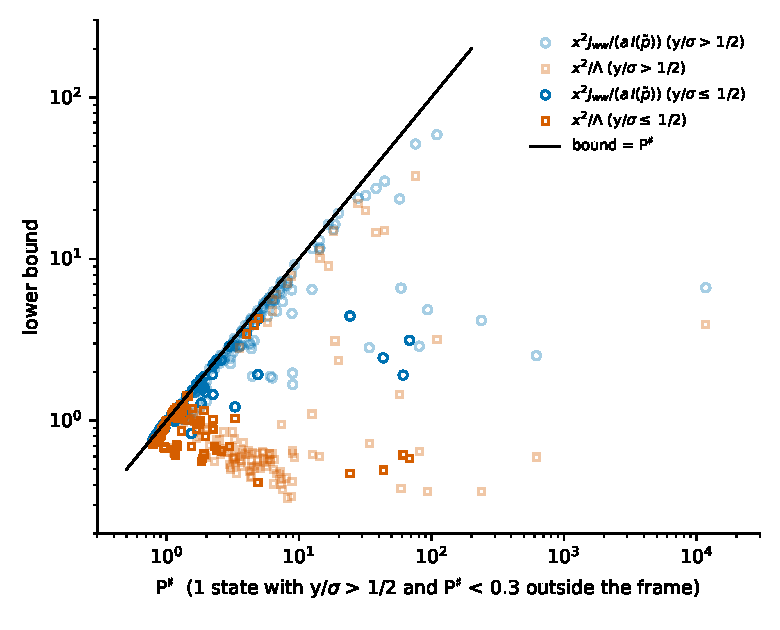
\includegraphics[width=0.85\columnwidth]{figures/figA1_chain.pdf}
\caption{The line route on 377 Gaussian mixtures: the lower bounds $x^2J_{ww}/(aI(\tilde p))$ (circles) and $x^2/\Lambda$ (squares) against the spread $P$ (denoted $P^\sharp$ in the axis label); dark symbols, focused states ($\Upsilon \leq 1/2$).}
\label{fig:chain}
\end{figure}

\begin{figure}[t]
\centering
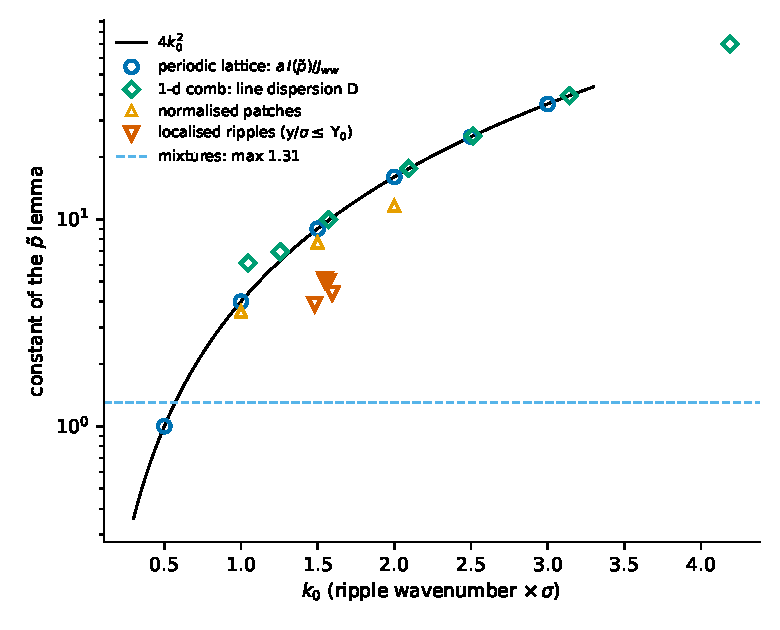
\includegraphics[width=0.85\columnwidth]{figures/figA2_families.pdf}
\caption{The constant of the line route on ripple families: periodic lattice and one-dimensional comb follow $4k_0^2$; normalised patches and localised ripples exceed the Gaussian-mixture maximum $1.31$ (dashed).}
\label{fig:families}
\end{figure}

\section{Numerical methods}
\label{app:methods}

\paragraph*{Gaussian mixtures.} Mixtures with up to $K = 32$ components were searched for small $g$, small $P$ and large values of the ratios of the line route, with the focus constraint $\Upsilon \leq 1/2$ imposed exactly. Each final state was re-evaluated on two grids of different resolution, and only states satisfying the constraint on both were kept. The smallest gap found, $0.884\,\sigma$ at $\sigma = 10^{-2}$, belongs to an ``hourglass'': a narrow needle at the top with weaker components spread along $w$. It was confirmed by three forms of the gap formula and by an independent quadrature written separately from the search code (relative difference below $5\times 10^{-4}$).

\paragraph*{Closed forms for the strips.} Each term of Eq.~\eqref{eq:strip} is a Gaussian in $w$ times, in $v$, either a Gaussian or the real part of $N(v;0,L_v^2)\,e^{ibv} = e^{-b^2L_v^2/2}N(v;\,ibL_v^2,\,L_v^2)$ with $b = k_0/\sigma$, a Gaussian with a complex mean. Blurs and posteriors of such terms are Gaussian with explicit means and variances, so that $\varrho$, $s$, $H$ and the posterior moments in Eq.~\eqref{eq:Ncov} are closed-form sums. The covariance in Eq.~\eqref{eq:Ncov} is evaluated with Stein's identity within each term and an explicit between-term part, in which all differences of nearly equal quantities are formed analytically. The fast phase $k_0 v/\sigma$ is integrated as an independent variable over one period at fixed slow position, with error of order (period$/L_v)^2$.

\paragraph*{Pitfalls.} Three effects produced wrong values in the course of the study and are guarded against in the final codes.
\begin{enumerate}
\item \emph{Rounding.} In the limit $\sigma^2/L_v^2 \to 0$, the matrix $I - \sigma^2 T^{-1}$ rounds to the identity in double precision, and a derivative computed from it carried a rounding error of $2\times 10^{-17}$ against a true value of $5\times 10^{-21}$. An earlier version of the study reported a floor of the strip gap at $0.234\,\sigma$ because of it. The derivative is now computed as $-\sigma^2 e_z\cdot T^{-1}e_p$, and a pointwise evaluation in 320-digit arithmetic agrees to $3\times 10^{-14}$ at $\sigma = 10^{-80}$.
\item \emph{Phase precision.} Positions written as an absolute coordinate plus a fraction of a ripple period lose the phase once $L_v/\sigma \gtrsim 10^{12}$. In that regime only phase-based evaluators are used.
\item \emph{Envelope aliasing.} Averaging one period at coarse slow positions aliases an oscillation of relative size period$/L_v$; at $\sigma = 10^{-6}$ this was a $3\times 10^{-3}$ error, found because a full two-dimensional grid and a phase-based evaluator agreed with each other but not with the third method.
\end{enumerate}
A lesson for the cross-checks: in the stage that produced the artefact of item 1, two evaluations with different integration schemes agreed because they shared the routine that computed the pointwise fields. Agreement between evaluations is evidence only if they share no code for the states, the pointwise fields and the integration. All values reported here satisfy this.

\paragraph*{Independent evaluation.} The strip values at $\sigma = 10^{-4}$, $10^{-6}$, $10^{-12}$, $10^{-24}$ and $10^{-48}$ were reproduced by an evaluator written separately from the closed forms above, with no code in common with the study. Its formulas for $\varrho$, $s$, $D$ and $\partial_p D$ were checked pointwise against direct two-dimensional quadrature of the posterior (relative differences below $10^{-6}$). It reproduced $g$ to ten digits or better, and an optimisation with it from unrelated starting points found $g_{\min} = 0.33487$ at $\sigma = 10^{-12}$ and $0.17938$ at $\sigma = 10^{-24}$, with the same optimal parameters.

\paragraph*{Fields of the heat-flow route.} The quantities of Sec.~\ref{sec:removing} ($J_{ww}$, $R$, $t^2R'$, the eigenvalues of $H$) were computed on two-dimensional grids from closed-form fields of mixtures and lattices. For the strips the curvature does not depend on the slow coordinate, so the largest eigenvalue of $-tH$ was taken over the full plane of the fast phase (720 points) and $y_w$ (about 5000 points) at 25 blurs; the maximum is unchanged when the region is restricted to densities above $10^{-8}$ or $10^{-12}$ of the maximum, and when the grid is refined. An earlier evaluation that took the maximum over quadrature nodes only gave $1.82$ instead of $1.87$. Separately from the study's code, the values of $-tH$ for the strip at $\sigma = 10^{-2}$ were reproduced on a two-dimensional Fourier grid of the state.

\paragraph*{Verification suite.} The repository (Data and Code Availability) contains the results, the figure scripts and a verification suite of 83 checks that recompute every number and inequality of this article from the stored results, with light recomputations: the hourglass minimum in three forms, a 320-digit pointwise check, the strip optima by two code-disjoint evaluators, the lemmas of Secs.~\ref{sec:direct}--\ref{sec:removing} on fresh test states. Every check reports the fraction of its tolerance that it uses; none uses more than $20\%$.


\section*{Acknowledgments}
The author used AI assistants in this work. OpenAI ChatGPT (\mbox{GPT-5.6 Luna}) and Google Gemini (\mbox{Gemini 3.8 Flash}) were each given the same draft for independent critical reading and cross-checking; this cross-check pointed out that the strips do not vanish outside the fundamental domain, which led to the moment conditions (H1) and (H2). Anthropic Claude (\mbox{claude-opus-5-5}) was used in two separate sessions. In the first session it took part in theoretical discussion, derived the gap formula (Proposition~\ref{prop:formula}) independently, wrote an independent evaluator of the strips, proposed the weaker target of Proposition~\ref{prop:target}, checked the proofs of the main results and reproduced key values (the strips and their valleys) by independent computations, and drafted the text. In the second session it designed and ran the numerical study, found the strips and the other families, derived Theorem~\ref{thm:direct}, Lemmas~\ref{lem:smoothing1d}, \ref{lem:heisenberg}, \ref{lem:split}, \ref{lem:fisher} and~\ref{lem:dip}, Theorems~\ref{thm:log}, \ref{thm:valley} and~\ref{thm:product} and Proposition~\ref{prop:novalley}, and wrote the evaluation and verification code. Results were passed between the sessions as written summaries and checked in the first session by re-running the verification suite and by independent methods. The author directed the research, made all decisions on its content, and takes full responsibility for this article.

\section*{Data and Code Availability}
Scripts, results and the verification suite that reproduce every number and figure of this article are openly available at \url{https://github.com/neginyan/resolution-gap-log-law}, together with independent checks and a notebook that reproduces the main numbers in a browser. The version used for this article is archived at Zenodo, \pending{code DOI}.


\begin{thebibliography}{99}

\bibitem{namba2026arrow}
T.~Namba, \textit{Sharp criterion for the coarse-grained arrow of time in Hamiltonian dynamics}, preprint, version v1.2, Zenodo (2026), \href{https://doi.org/10.5281/zenodo.23258135}{doi:10.5281/zenodo.23258135}.

\bibitem{namba2026gap}
T.~Namba, \textit{A resolution gap for the coarse-grained arrow of time in nonlinear Hamiltonian flows}, preprint, version v1.1, Zenodo (2026), \href{https://doi.org/10.5281/zenodo.23320603}{doi:10.5281/zenodo.23320603}.

\bibitem{namba2026many}
T.~Namba, \textit{The resolution gap in many degrees of freedom}, preprint, version v1.0, Zenodo (2026), \href{https://doi.org/10.5281/zenodo.23371932}{doi:10.5281/zenodo.23371932}.

\bibitem{namba2026learned}
T.~Namba, \textit{Can a learned score see the margin of the arrow of time?}, preprint, version v1.0, Zenodo (2026), \href{https://doi.org/10.5281/zenodo.23408213}{doi:10.5281/zenodo.23408213}.

\bibitem{namba2026threshold}
T.~Namba, \textit{A stretching-rate threshold for phase-space diffusion models with isotropic marginal noise schedules}, preprint, Zenodo (2026), \href{https://doi.org/10.5281/zenodo.23181225}{doi:10.5281/zenodo.23181225}.

\bibitem{dockhorn2022}
T.~Dockhorn, A.~Vahdat, and K.~Kreis, \textit{Score-based generative modeling with critically-damped Langevin diffusion}, in \textit{International Conference on Learning Representations} (2022).

\bibitem{efron2011}
B.~Efron, \textit{Tweedie's formula and selection bias}, J. Am. Stat. Assoc. \textbf{106}, 1602 (2011).

\bibitem{folland1997}
G.~B. Folland and A.~Sitaram, \textit{The uncertainty principle: a mathematical survey}, J. Fourier Anal. Appl. \textbf{3}, 207 (1997).

\bibitem{cover2006}
T.~M. Cover and J.~A. Thomas, \textit{Elements of Information Theory}, 2nd ed. (Wiley, Hoboken, 2006).

\bibitem{bakry2014}
D.~Bakry, I.~Gentil, and M.~Ledoux, \textit{Analysis and Geometry of Markov Diffusion Operators} (Springer, Cham, 2014).

\bibitem{toscani2015}
G.~Toscani, \textit{A concavity property for the reciprocal of Fisher information and its consequences on Costa's EPI}, Physica A \textbf{432}, 35 (2015).

\bibitem{kannan2026}
J.~B. Kannan, S.~PG, and M.~S. Santhanam, \textit{Probing chaos and criticality with observational entropy and finite-resolution measurements}, arXiv:2605.23585 (2026).

\end{thebibliography}


\end{document}
